\documentclass[12pt]{article}
\usepackage{fullpage}
\usepackage{subcaption,amsmath,amssymb,mathtools,xparse,graphicx,float,datetime,color,array,graphics,enumerate,tikz,pgfplots,xcolor}
\usepgfplotslibrary{statistics}
\pagestyle{empty}
\newcommand{\D}{\displaystyle}
\setlength{\textheight}{9in} \setlength{\headheight}{.2in}
\setlength{\headsep}{0in} \setlength{\topmargin}{0in}
\begin{document}
\begin{center}
CSCI 6100 Machine Learning From Data\\
Fall 2018\\
\end{center}
\begin{center}
HOMEWORK 11\\
Daniel Southwick\\
661542908\\
southd@rpi.edu
\end{center}
\vspace{.1in}

\noindent {\bf 1. k-NN Rule} \\\\
\noindent a)\\
\indent We first randomly selected 300 datas out of the Number 1 and Number 5 data as our training set, and use the remaining as our testing set. Using the same feature from HW9, the selected data is shown below:
\begin{figure}[H]
  \centering
  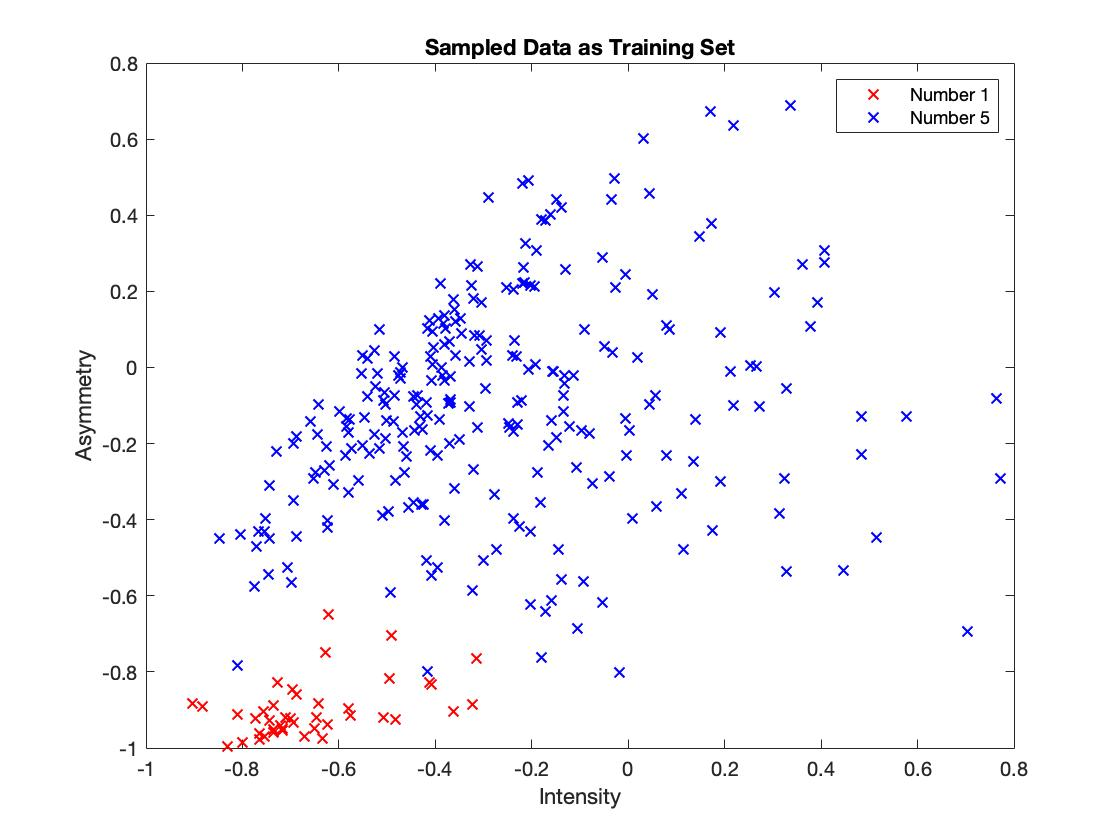
\includegraphics[scale = 0.27]{1.jpg}
  \caption{300 Samples as Training Set}
  \label{fig:1}
\end{figure}
\indent We then run the training data set through different kNNs training model, with k ranges from 0 to 200. During each training, we computed the different cross validation error. The minimum cross validation came out to be $0.08\%$, it is found at when $k = 16$. So we take $k = 16$ as our optimal $k$.
\begin{figure}[H]
  \centering
  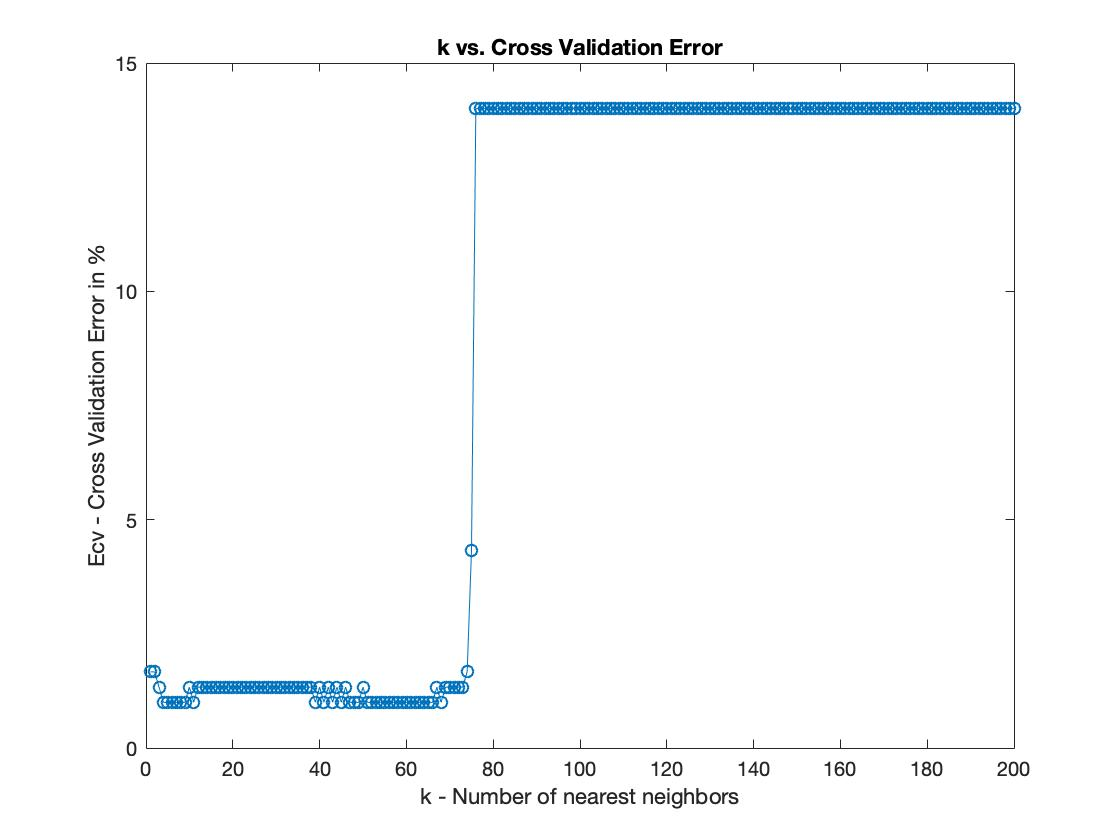
\includegraphics[scale = 0.27]{2.jpg}
  \caption{k vs. Cross Validation erros for kNN}
  \label{fig:2}
\end{figure}
\noindent b)\\
\indent The 16-NN decision region is shown below. We find the 16 nearest neighbors and get its corresponding classification for each dataset. The in-sample error came out to be $0.067\%$ and The cross validation error is $0.08\%$.
 \begin{figure}[H]
  \centering
  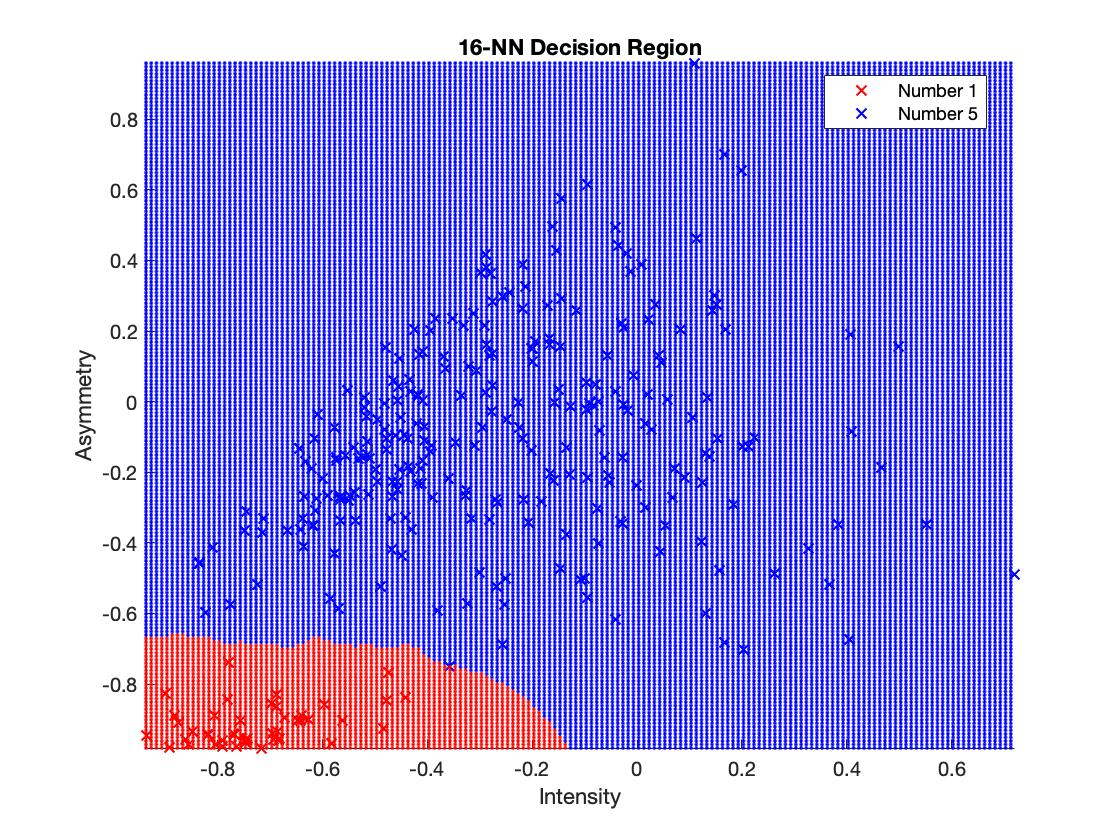
\includegraphics[scale = 0.27]{3.jpg}
  \caption{16-NN decision region}
  \label{fig:3}
\end{figure}
\noindent c)\\
\indent We then run the test data set, $8998$ data points, on our 16-NN model, the test error came out to be $1.57\%$. So this is a good fit for the Num 1 and Num 5 data set.

\newpage
\noindent {\bf 2. RBF-network} \\\\
\noindent a)\\
\indent Similar to HW10, we apply Lloyd's Algorithm to find the $k$ centers of the input data. We compute the error during each iteration by: $\displaystyle \sum_{i = 1}^{300}||x_i-\mu(x_i)||^2$, where $\mu(x_i)$ are the centers during each iteration. We update these centers until $\displaystyle (\sum_{i = 1}^{300}||x_i-\mu(x_i)||^2)_k - (\sum_{i = 1}^{300}||x_i-\mu(x_i)||^2)_{k+1} \leq 0.1$. \\\\
\indent For each different number of centers, $k$, we compute the cross validation error by summing up the weights of each training data to the centers, with the weights computed using Gaussian functions $\displaystyle \phi(\frac{||x_i - x||}{r}), r = \frac{2}{\sqrt{k}}$, where $x$'s are the different centers. We compare the estimated class in the 300 sample, count the number of difference with the actual class, then we divided by 300 to get the cross validation error. The errors with different k's are shown below:
\begin{figure}[H]
  \centering
  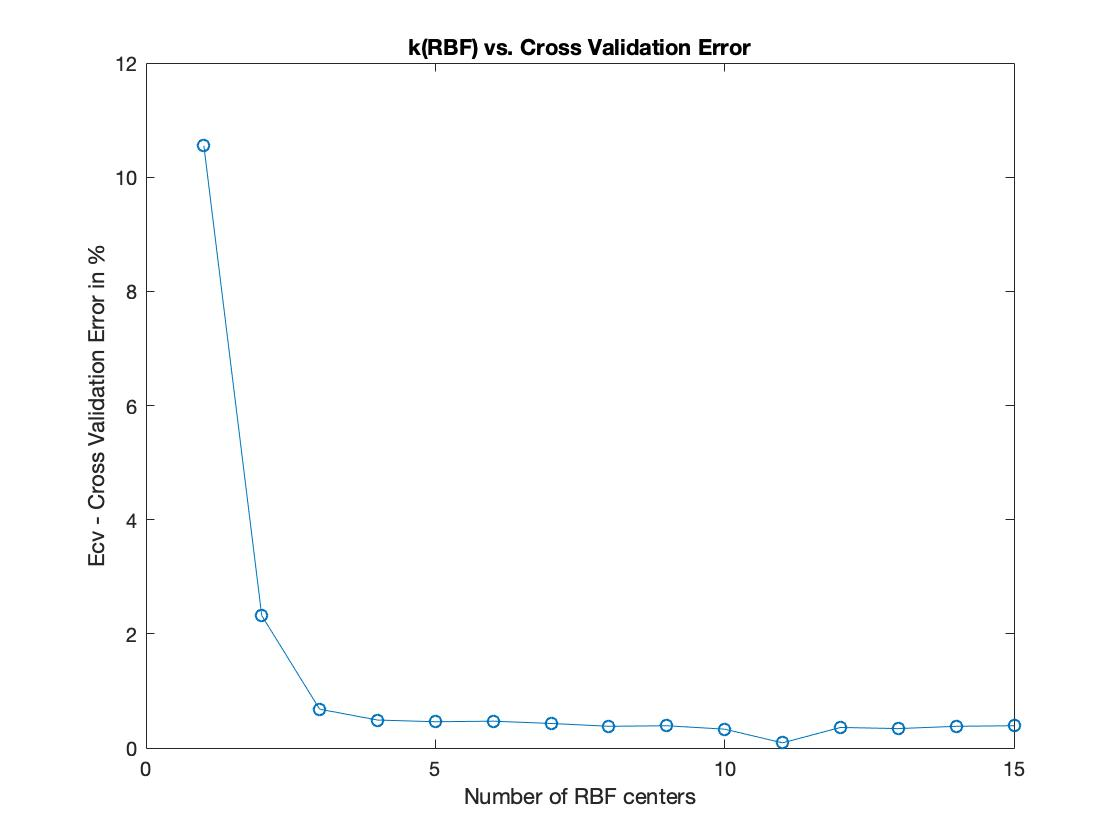
\includegraphics[scale = 0.27]{4.jpg}
  \caption{k vs. Cross Validation erros for RBF}
  \label{fig:4}
\end{figure}
\indent The minimum cross validation came out to be $0.03\%$, it is found at when $k = 11$, so we take $k = 11$ as our optimal $k$.\\
\newpage
\noindent b)\\
\indent The RBF network with Gaussian kernel with $k = 11$'s decision region is show below. The in sample error came out to be $0\%$ and the cross validation error is $0.03\%$
\begin{figure}[H]
  \centering
  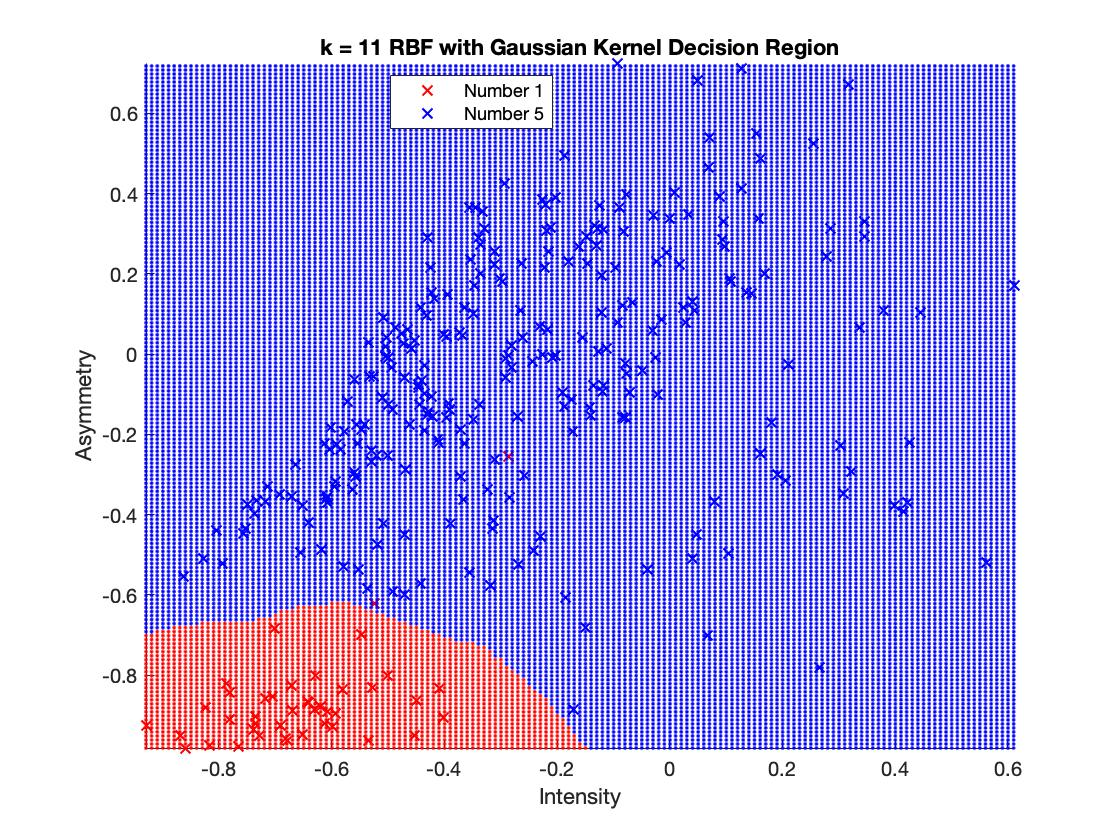
\includegraphics[scale = 0.27]{5.jpg}
  \caption{k = 11 RBF decision region}
  \label{fig:5}
\end{figure}
\noindent c)\\
\indent Again, we run the test data set with our model, the test error came out to be $0.85\%$\\\\

\noindent {\bf 3. Compare Linear, k-NN, RBF-network} \\\\
\indent We have computed the Linear model with 8th order polynomial transform and regularization in HW9, and we recall that the test error is $0.9\%$.  All the method above has similar test error rate, and they all seems like good fits to the data set. In this case, RBF network with Gaussian kernel has the lowest test error. Though RBF performed better, in general, k-NN algorithm has a much lower computation cost than linear feature transform and RBF network, so I would go with k-NN algorithm to get the best result if an unknown data set is given.

\end{document}

